% Chapter 4

\chapter{Deoptimization in RJIT} % Main chapter title

\label{Chapter4} % For referencing the chapter elsewhere, use \ref{Chapter4} 

%----------------------------------------------------------------------------------------

% Define some commands to keep the formatting separated from the content 
\newcommand{\keyword}[1]{\textit{#1}}
\newcommand{\tabhead}[1]{\textbf{#1}}
\newcommand{\code}[1]{\texttt{#1}}
\newcommand{\file}[1]{\texttt{\bfseries#1}}
\newcommand{\option}[1]{\texttt{\itshape#1}}

%----------------------------------------------------------------------------------------
NOT SATISFIED WITH THE PLAN FOR THE MOMENT: TRY JUSTIFICATION, DEOPTIMIZATION, REAL API FOR OSR RJIT, POSSIBLE EXTENSIONS AND PROTOTYPES.\\

This chapter presents our design to support OSR transitions and OSR deoptimizations in LLVM, and more particularly in the RJIT project.
Our design and implementation is based on OSR Kit\cite{OSRKit, OSRKitGit}, an OSR library for LLVM, implemented by \citean{OSRKit} at the department of Computer, Control, and Management Engineering of the Sapienza University of Rome.
This implementation provides several features of existing techniques, that were never simultaneously supported in a single framework.
It is flexible enough to be used to implement our own model for OSR deoptimization.
We therefore decided to use and extend it, in order to provide OSR deoptimization for R.\\

\section{Overview}
This section presents our goals for this Master Thesis Project and justifies the use of the OSR Kit as the base of our OSR support in RJIT.\\

%TODO MAYBE switch the Justification and the LLVM Library

\subsection{Justification}
%Our goal: OSR deoptimization for R.
    %R has shitty performances
    %need aggressive optimizations
    %Work with the rjit project, so based on LLVM. 
    %Too soon to know what we really want, so need a mechanism as flexible as possible.
%What do we want form OSR Kit? 
    %A transition mechanism
    %An LLVM library that is mostly optimization and language independent.
        %Why? Because we want to work at the LLVM IR level, which is stable.
%Why not from scratch?
    %Reinventing the wheel seems like a waste of time. 
    %Enables to focus on deoptimization case.
    %Enables to test a proper optimization. 
    %Can extend it with new features, can modify it.
The goal of this Master Thesis project is to provide a flexible OSR deoptimization framework in LLVM, and use it to improve performances in RJIT, our LLVM JIT compiler for R.
R is a programming language and software environment for the statistical computing and graphics, developed by the R Foundation for Statistical Computing\cite{RURL}.
Due to SAY WHYYYYYYYYYYYYYYYYYYYYYYYYYY OOOOOHHHHH GOOOOOOODDDDDD WHHHYYYYYYYYYY, R exhibits very poor performances CITE SOMETHING.
The RJIT project strives to improve these performances by providing a LLVM based JIT compiler for R. SAY MORE.
The RJIT compiler is still pretty young, only a few months old.
As a result, we lack FEEDBACK; DONT KNOW EXACTLY HOW TO IMPROVE PERF AND NEED TO EXPERIMENT.
Therefore, we are looking for a flexible and extensible OSR mechanism that enables us to prototype and experiment various solutions, without trapping ourselves into a single model.\\

The OSR Kit library\cite{OSRKit} is a flexible implementation of on-stack replacement instrumentation in LLVM.
The source-code for the library is available on Github\cite{OSRKitGit}, and the library can be used in any LLVM project by simply copy-pasting the OSR Kit files inside of it.
The simple integration, the availability of the source code, and the flexibility of the framework make it a perfect base implementation upon which we can implement our support for OSR deoptimization mechanisms in RJIT.\\

%TODO MORE ABOUT THE FOCUS ON DEOPT.
This master project thesis focuses on the design and implementation of a prototype for OSR deoptimization support in RJIT.
Starting a new OSR transition implementation from scratch requires time.
Using a flexible and modifiable OSR transition library therefore seemed like the goto option.
We do not waste time reimplementing something that already exists, and can therefore put all our efforts into implementing an interesting OSR deoptimization case, testing it, and extending the OSR Kit library with mechanisms that are specific to our needs (Sections \ref{osrForUs} and \ref{extendingOSR}).\\

\subsection{An LLVM Library}

The OSR Kit is a general-purpose, target-independent, implementation of on-stack replacement for LLVM.
As such, it can be used by any LLVM based compiler.
The main goals of the OSR Kit project are:
\begin{enumerate}
    \item To allow chained OSR transitions, i.e., a continuation function can be instrumented to allow OSR transitions.
    \item To support OSR entries and exits via the same instrumentation.
    \item To allow transitions at arbitrary function locations.
    \item To allow continuation functions to be either generated at run time, or already known at compilation time (i.e., generated on the fly or cached).
    \item To encapsulate and hide the OSR implementation details from the front-end.
    \item To encode OSR transitions entirely at the LLVM IR level.
    \item To limit the intrusiveness of the OSR instrumentation.
    \item To allow the LLVM's compilation pipeline to generate the most efficient native code for an instrumented function. \label{llvmTransformPasses}
\end{enumerate}

%2 means that what the framework really provides is a transition mechanism. 
%3 leaves the responsability to the user to id potential transition points
%4 we have both the generated on the fly and the cached semantics, enables us to test both.
%6 Stable representation
%8 This point is important in our case study Chapter 5, inlining mostly to extend the scope of possible optimizations.
%MORE about it being a tool and the OSR is left to the user.
The OSR Kit library's main contribution is the implementation of an efficient and flexible OSR transition mechanism.
This transition can be used to implement OSR entries and OSR exits alike.
Allowing OSR points to be inserted at any location enables the user to experiment with the OSR mechanisms at any instruction boundary. 
In other words, the OSR library is designed to give the user as much freedom as possible.
Section \ref{tradeOffs} explained the basic trade-offs between generating the continuation function on the fly and caching already compiled versions.
Where other implementations, such as McOSR\cite{lameed2013modular}, made a clear choice between the two techniques, the OSR Kit library decided to enable both of them, hence allowing the user to experiment and select the design that better suits specific use cases.\\

%TODO MISSING FROM NEW
LLVM IR is a stable representation that combines the advantages of both the high-level representation, i.e., it still contains some semantic constructions particular to the language being compiled, and the advantages of a lower level representation, closer to the execution engine.
In the case of this master thesis project, i.e., providing OSR mechanisms in the RJIT project, the LLVM IR is the exact middle layer representation that we need. 
The R AST representation is too high level and prevents us from introducing efficient OSR instrumentation. 
At the LLVM IR level, the R semantics are still visible and it therefore allows us to efficiently implement our optimizations.\\

Point \ref{llvmTransformPasses} is important in order to leverage the full power of the LLVM transformation and optimization passes.
One of the main advantages of using the LLVM framework is that LLVM transformation passes and optimizations can be automatically added to the compilation pipeline in order to improve the quality of the code generated.
For example, in the case study in Chapter \ref{Chapter5}, one of the OSR inlining mechanism's goals is to extend the scope in which the LLVM passes run in order to improve the code quality.\\


\section{Resolved \& Open OSR}
The OSR Kit library\cite{OSRKit} provides the choice between generating the continuation function of an OSR transition on the fly, or using an already compiled function.
This section describes both techniques as they are implemented in the OSR Kit library.\\
 
\subsection{The Open OSR}
%Generate on the fly.

%How it works
    %theory
    %practice

%Ok for optimizations
%Less okay for deoptimization.
The \textit{open OSR} scenario corresponds to the case where the continuation function is generated when the OSR transition is fired.
Deferring the compilation of the continuation function allows profiled-guided compilation strategies to gather as much information as possible about the current state of the execution, and therefore generate the best possible code.\\

The open OSR scenario is implemented as a call to a stub function, call it $f_{stub}$.
The $f_{stub}$ function is responsible for generating the continuation function, and then transferring the execution to it.
The continuation function is generated by a special \textit{gen} function, that takes as inputs the base function $f$, i.e., the from function, and the OSR point that triggered the transition.\\
%TODO code for the OSR points open. 

Figure REF corresponds to the signature of the OSR Kit function that enables to insert open OSR points.
The \textit{destFunGenerator} is the $f_{stub}$ function and is of type \textit{DestFunGenerator}, described in Figure REF.\\

\begin{minipage}{\linewidth}
\includecode{Code/DestFunGenerator.c}
\end{minipage}

\begin{minipage}{\linewidth}
\includecode{Code/OpenOSR.c}
\end{minipage}

%TODO MISSING FROM NEW
Open OSR are hard in the deoptimization case.
Being able to generate a continuation function on the fly for an OSR exit requires the framework to be able to undo an optimization.
The RJIT framework, does not, for the moment, provide means to keep track of transformations performed on a function, and efficiently revert them.
For example, the VARMAP data structure in the Jikes RVM OSR implementation\cite{soman2006efficient} is automatically updated by the framework when a transformation is performed on the function.
This enables to reverse the steps that lead to the optimized version.
While the RJIT compiler does not provide such mechanism, we could imagine keeping the LLVM IR of the original function in memory, without compiling it.
When an open OSR exit is triggered, the unoptimized LLVM IR for the function is retrieved, the continuation point is identified, and RJIT instruments and compiles the correct continuation function.
This solution enables to avoid the cost of going through the entire compilation of the continuation function until it is truly needed.
On the other hand, it increases the amount of work performed during the OSR transition.\\
%TODO add a sentence to say if it is tested or not in our implementation
%In order to do so, we have a handler, that keeps the version etc., 
%So I guess I'm gonna try it.

\subsubsection{Similarities with McOSR}
The open OSR is similar, in theory, to the McOSR implementation\cite{lameed2013modular}.
Both of them rely on a \textit{gen} function to generate the continuation function when the OSR transition is fired.
However, \citean{OSRKit} made the choice to perform these operations, i.e., generating the continuation function and transferring the execution, inside a separated function, rather than instrumenting the from function directly.
This choice was made in order to minimize the code injected inside the from function.
In fact, the instrumentation, even when inserted in a separated branch, might interfere with compiler optimizations.
Examples of such interferences are the increase of register pressure, the alteration of code layout and instruction cache behavior.\\

\subsection{The Resolved OSR}

The \textit{resolved OSR} scenario corresponds to the case where the continuation function is known prior to fire the OSR transition, and the from function has been instrumented to transfer the execution to this specific continuation function.
In the resolved OSR scenario, the transition is expected to be faster than in the open scenario, since there is no compilation to be performed. 
This technique also enables to reuse functions that were compiled previously, e.g., either because several from functions have the same continuation function, or because an OSR point is fired several times during the execution of the program.\\

The resolved OSR is implemented as a call to the continuation function, which takes as inputs all the live variables at the OSR point as inputs.
The continuation function is instrumented to jump at the correct location inside the code to resume the execution. 
Figure \ref{ResolvedOSRFig} illustrates the resolved OSR scenario.\\

\begin{figure}[h]
\centering
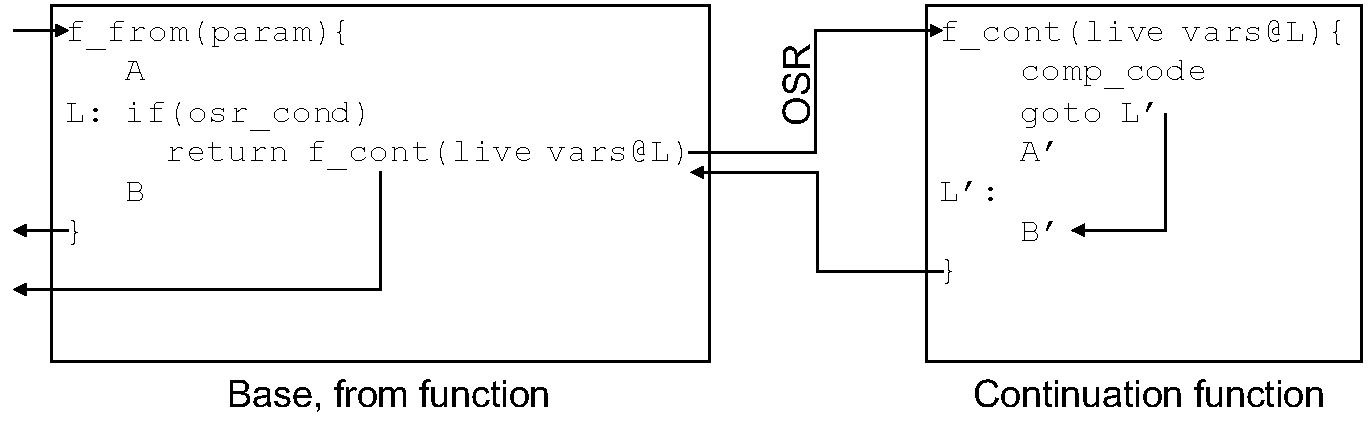
\includegraphics[scale=0.5]{Figures/OSRKitResolvedScenario}
\decoRule
\caption[Resolved OSR Scenario]{Resolved OSR scenario, from\cite{OSRKit}.}
\label{ResolvedOSRFig}
\end{figure}

Figure REF corresponds to the signature of the OSR Kit function that enables to insert resolved OSR.\\

\begin{minipage}{\linewidth}
\includecode{Code/ResolvedOSR.c}
\end{minipage}

%TODO MISSING FROM NEW
The resolved OSR scenario does not require to inverse on the fly the transformations performed on the function and can therefore easily be used to implement the deoptimization case.
In order to obtain the optimized version of a function, one has to perform transformations on a base function.
This base function can therefore be used as the continuation function in the case of an OSR exit.
In RJIT, we rely on the resolved OSR to provide deoptimization of functions where call sites were inlined.
While generating the optimized version by speculatively inlining calls, the RJIT compiler introduces the OSR exit instrumentation with the base function as continuation function.
When several call sites are inlined, each of them is instrumented with an OSR exit that points to its own continuation function, which is a copy of the base function with the proper OSR instrumentation (see Section \ref{thecontinuationfunction}).\\



\section{The OSR Instrumentation}
\subsection{OSR Points \& Conditions}
%No distinction
%Both are done in the same way i.e., insert a condition.
%Do the condition testing, do the jump to a special block.
%Requirements for the point to be inserted !

In the OSR Kit library\cite{OSRKit}, there is no distinction at the implementation level between OSR exits and entries.
The general mechanism used is the OSR point.
An OSR point corresponds to a labelled LLVM basic-block that contains the call to the continuation function and the return instruction to propagate the result of the call.
OSR points are protected by an OSR condition. 
The OSR Kit library allows an OSR condition to be any vector of LLVM instructions. 
The last instruction is automatically used by the framework as condition for an LLVM branch instruction. 
If the condition succeeds, the OSR transition is fired.
Otherwise, the execution continues in the function.\\

Figures REF and REF provide an example of OSR instrumentation.
In Figure REF, we have the R declaration of two functions, $f$ and $g$, and the simplified LLVM IR generated for $g$ in RJIT.
Figure REF presents the instrumented version of $g$, in which an OSR point has been inserted.
Lines 5 and 6 correspond to the OSR condition.
In this example, the OSR is fired if line 1 does not yield the same function for $f$ as the one that was used by the RJIT compiler when it generated the instrumented function.
If the OSR is fired, the execution jumps to the \textit{OSR\char`_fire} basic block and calls the continuation function, namely \textit{OSRCont}.
The OSR point \textit{OSR\char`_fire} calls the continuation and propagates its return value line 15.
The \textit{OSR\char`_split} block corresponds to the regular continuation of the function $f$ when the OSR is not fired.\\

\begin{minipage}{\linewidth}
\includecode[asm]{Code/original.llvm}
\end{minipage}

\begin{minipage}{\linewidth}
\includecode[asm]{Code/fromInstrumented.llvm}
\end{minipage}

%TODO Requirements for a point.
REQUIREMENTS FOR OSR POINT\\

\subsection{The StateMap}

The OSR Kit library and our extensions heavily rely on a special object, called a \textit{StateMap}, to keep a mapping between the from function and the continuation function.
The StateMap enables to register unidirectional and bidirectional mappings between LLVM instructions and function arguments.
The default constructor for a StateMap relies on the LLVM ValueToValueMapTy\cite{VMap}(VMap) to automatically extract the mappings.
A VMap can be filled with such mappings when the LLVM cloning functions are used, i.e., the OSR Kit encourages you to generate the continuation function by cloning either the base or the from function such that a VMap is already available when the framework needs to introduce the instrumentation.
The StateMap also provides an API to register and unregister mappings by directly providing the two instructions.\\

%Transitive mappings
%Enables to skip versions!
%TODO MISSING FROM NEW
In order to facilitate the use of StateMaps in the deoptimization case, we extended the object with transitive mappings.
Suppose two StateMaps, $S_1$ and $S_2$, such that $S_1$ is a mapping between $A$ and $B$, and $S_2$ a mapping between $A$ and $C$.
Our transitive constructor will be able to generate a new StateMap, $S_3$, that maps $B$ and $C$.
Consider a chained generation of versions, i.e., a succession of versions where each one of them is the result of some transformation applied on the previous version.
$$A \rightarrow B \rightarrow C \rightarrow D \rightarrow E \rightarrow F \rightarrow ...$$

The transitive StateMap constructor enables to automatically generate a transitive map between each versions in the chain.
The StateMap might not be complete, but it ensures that every instruction that is present in the base version $A$ and both versions that we want to map, e.g., $C$ and $F$, will be present in the StateMap.
WHY IT IS USEFUL !!!

\subsection{The continuation function}\label{thecontinuationfunction}
%The continuation function same in principle if we come from open or resolved. 
%Replaces the entry point of the function with a special OSR_ENtry block.
%CODE example
%block responsible for compensation code and jumping to the correct instruction, which is instrumented by the framework to be the head of a basic block. Everything before is deadcode, eliminated by LLVM automatically if optimizations are enabled.

%Live values are passed as arguments so no need to do any loading. Speed up the whole thing: quote from paper.

%In optimization -> optimize long running functions that's okay. Frequently called functions, a bit less. WHY
%In deoptimization, that is perfect if we do not expect to deoptimize frequently. 
%Got rid of that in RJIT by allowing the comp code to reset the closure corresponding to the function to actually contain the full deoptimzed method. TADA This is in the handler (see section bla). 

Both deoptimization and optimization rely on the same kind of continuation functions, and on the same instrumentation tools.
A continuation function, in OSR Kit, has a special function signature that takes as inputs all the variables that were live at the instruction at which the OSR transition was fired.
Its return type is the same as the from and the base (unmodified and un-instrumented) functions.
The OSR Kit instrumentation inserts a special basic block, called \textit{OSR ENTRY}, at the beginning of the continuation function.
The OSR ENTRY is responsible for executing a compensation code and jumping to the correct block inside the continuation function.
The compensation code is specified by the library user as a vector of instructions, when the OSR is inserted in the code.
The continuation instruction, i.e., the instruction to which the OSR ENTRY jumps to is assured by the OSR Kit library to be the first instruction in the destination block.
Everything between the OSR ENTRY and the continuation block becomes considered dead code.
The dead instructions are automatically eliminated by the LLVM transformation passes.
In any case, their only impact is on the space used up by the program, their presence does not increase the execution time of the continuation function.
It might, however, impact on later optimizations performed on the code.\\

CODE EXAMPLE.\\

Passing live values as arguments to the continuation function is more efficient than loading them from a buffer.
According to \cite{fink2003design}, generating a dedicated function to resume the execution to continue the execution, as opposed to instrument a general function to serve as continuation as well as a regular function, is expected to lead to better results.
In other words, it is supposed to be better to keep the base function to serve regular calls, and trigger OSR transitions whenever we need them, during the execution of the function.\\

%TODO Missing from new
In the case of long running functions, generating this type of OSR continuation function to transfer the execution to a more optimized version of the code makes sense.
The OSR entry is usually fired at some special control flow node, such as a function prologue or a loop header.
Therefore, the code expected to be repeatedly executed is not dead inside the continuation function.
On the other hand, the code leading to that portion, i.e., the code that needs to be executed only once or a few times, is dead code and does not matter.
It can therefore be removed without regret.
On the other hand, if the function is not a long running one, going through the cost of compiling the continuation function might overcome the benefits of the optimization. 
Nevertheless, if that is the case, a JIT compilation of the function should be used instead of the OSR mechanism.
If the optimization is based on an assumption that might fail, one can always JIT compile it with optimizations, and instrument it with OSR exits.\\

In the case of deoptimization, performance is a soft issue.
OSR exits are responsible for preserving correctness in the program. 
If an OSR exit is fired, the continuation function will be called.
Subsequent calls are still served by the optimized version of the function and might need to OSR exit too.
This can lead to a serious loss of performances.
For example, in the case of speculative call site inlining, an OSR exit is taken when the inlined function is redefined.
In subsequent calls, the same OSR exits will have to be taken.
With the OSR exit, the execution goes through an extra function call and return than in the unoptimized version.\\

In RJIT, when we know that an optimized version is no longer valid and will not be valid for subsequent calls either, we use the compensation code at the beginning of the continuation function to replace the optimized function in the environment with its unoptimized version.
The unoptimized version is a clone of the continuation function without the OSR instrumentation and with the same signature as the base function.
This mechanism is detailed in REF.
If we take the inlining example above, replacing the function with one that does not wrongly inline the call site is supposed to lead to better performances.\\


\section{Using OSR Kit to deoptimize}\label{osrForUs}
MIGHT MOVE THAT SOMEWHERE ELSE\\
\subsection{A case that does not fit perfectly}
PRESENT WHAT WE NEED TO CHANGE IN OSR KIT AND THE CHALLENGES.\\
%Cannot apply opposite of transformation so need to keep the base version somewhere. 
%Exit must be known in advance.
%Need to generate a lot of IR for a single function. 
%The OSR kit library works with a special continuation that cannot be used for regular calls, so need to be able to get this representation at some point for deopt and replace it.

%RJIT and the constants, instrumentations and other stuff on the side that makes it more difficult than just copying around the IR.
%Requires to clone a lot so increase the time spent in the compiler.
%One trick is to keep track of everything and reuse it as much as possible.

%Closures and what that implies. 
%Replacing the function. 

%As a conclusion, not exactly what we need here
Using OSR Kit to implement OSR based deoptimization in RJIT presents important trade-offs.
On one hand, generating a transformation that removes optimizations is hard.
It is easier to know where to exit in advance.
As a result, we need to keep track of the base function on which the optimization was applied. 
This fits the OSR Kit library's resolved OSR style, i.e., the continuation function is simply the base version that we used to generate the optimized one, and we can insert a resolved OSR when we perform the optimization.
On the other hand, this way of generating the continuation function is expensive, especially for deoptimization.
First, it requires to obtain two copies of the same base function, i.e., one to transform, and another that will serve as the continuation function.
Since the continuation function's signature might not be the same as the base function's one, the OSR Kit framework will perform a clone of the body of the function. 
Assuming we perform the optimizations on the base function, that still leaves us with two clones of the function per OSR point inserted.
Finally, as mentioned earlier, the fact that the continuation function is unable to serve regular calls implies that whenever the optimized function is deemed useless, i.e., any call to it will trigger an OSR exit, an un-instrumented version of the base function has to be compiled to serve regular calls.

In summary, the OSR Kit library's way of generating the continuation fits the RJIT requirements, but is costly and requires extra work when an assumption fails.
Section REF presents the OSR Handler, which enables to keep track of versions generated and decreases the amount of compilation required inside RJIT.\\

In RJIT, LLVM attributes\cite{llvmAttribute} associated to the LLVM IR are used to generate the safepoints for the call stubs and the garbage collector.
For example, when a call stub is inserted inside a function, a patchpoint identified by a unique id is inserted as an LLVM attribute in the corresponding call instruction, and registered inside the framework as a patchpoint that needs special instrumentation in the final compilation steps.
If not properly set, the call stub will not be resolved at run time and lead to unexpected behaviors.
As a result, simply cloning LLVM IR that corresponds to an R function is not enough.
Patchpoints and attributes also need to be fixed. 
As explained before, the OSR Kit library requires to generate several clones of the function on which we perform transformations. 
The RJIT framework therefore has to fix patchpoints and attributes for any of these clones that might be called during the execution.\\

 
\subsection{Where to exit?}
%What is possible and what is not
%Well can only exit to the previous version by default. BY DESIGN. 
%RJIT and transitive allow to make that more flexible, e.g., imagine there inlining
%Requires remapping of live values too.
The OSR Kit library, by design, encourages the OSR exit to target the base version that was used to generate the optimized one.
The insertResolvedOSR requires to provide a StateMap as input.
As explained in REF, the StateMap can either be automatically generated while cloning a function, or filled up by hand. 
The RJIT framework does not provide enough analysis information for the moment to be able to generate a StateMap from scratch, to map two different functions.
As a result, we keep the ...

\section{Extension in OSR RJIT}\label{extendingOSR}
%In this section details novel implementations, some of which we're referenced above.
%Added on top of the osr kit library, enables to better fit our use cases and also to enable to 
%switch from one design to another, experiment with different solutions etc. 

\subsection{The OSR Handler and function versions.}
%Takes care of the cloning and versioning 
%Provides simplified API to insert OSR points.
%Keeps track of statemaps.  
%Provides methods to update the statemap as we go, simple remove entries and add entries for now. 
%Future: would be great to have it wrap around the LLVM function and do all of that automatically, but that is a huge amount of work that we do not provide yet. 

\subsection{Fusing versions?}
%TRANSITIVE STATEMAPS
%Why do we want that ?
%it is a first step toward one continuation function, i.e., we can have the buffer implementation more easily 
%invalidate several assumptions at the same time -> e.g. inlining at the same level + reduces the number of versions that we keep in memory. 
    %What about the function signature? => take both sets and get union of them in the function signature, patch them will null values if they are not needed during the call. 
    %Implementation status .... wolololo


\subsection{Unguarded OSR points?}
%Keep track of stackmaps and patchpoints -> can enable this 

